
\chapter{}
\label{app:SI2}

\begin{figure}
\includegraphics[width=\linewidth]{../figures/appB/557_ideal_gcn.pdf}
\caption{A graph of the generalized coordinate number of an ideal Pt (557)
system colored to match the inset figure. Other than the bulk (GCN=12), the
(557) surface displays three primarily different surface sites, the edge atoms
(red, GCN=5.5), the plateaus (orange, GCN=7.2,7.5) and the slightly eclipsed
atoms beneath the step (yellow, GCN=8.7). Subsurface atoms have a larger GCN
than the surface atoms, but are still less than the bulk GCN of 12.}
\label{fig:557GCN}
\end{figure}


\newpage

%\begin{figure}
%\includegraphics[width=0.4\linewidth]{../figures/supportingInformation/}
%\caption{}
%\label{}
%\end{figure}
%\newpage


\begin{figure}
\includegraphics[width=0.4\linewidth]{../figures/appB/112_sunken.pdf}
\caption{The (112) systems, because of their large surface energy underwent a
minor refaceting that resulted in many of the (100) steps sinking slightly into
the surface (white). A few step edges (lime) retained their (100) step edge
morphology and were often the source for adatom formation.}
\label{fig:112sunken}
\end{figure}
\newpage


%\begin{figure}
%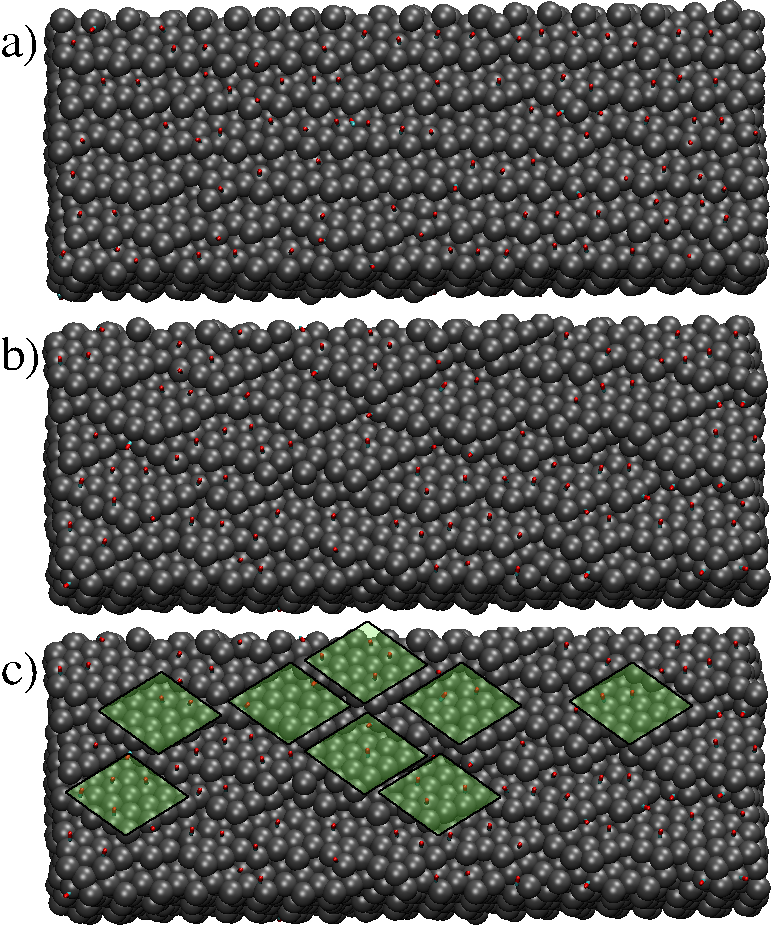
\includegraphics[width=0.8\linewidth]{../figures/appB/321MiniDiamonds}
%\caption{The energy required to translocate a kinked atom along the step edge
%is minimal, and on the (321) surfaces this leads to the formation of numerous
%small (111) diamonds on the surface. Systems are shown at (a) the beginning and
%(b)-(c) the end (100 ns) of the simulation for the (112) LS 0.25 ML system.
%While some step-edge doubling is observed, a significant portion of the surface
%has been replaced with these small diamond domains.}
%\label{fig:321Diamonds}
%\end{figure}
%\newpage







\begin{figure}
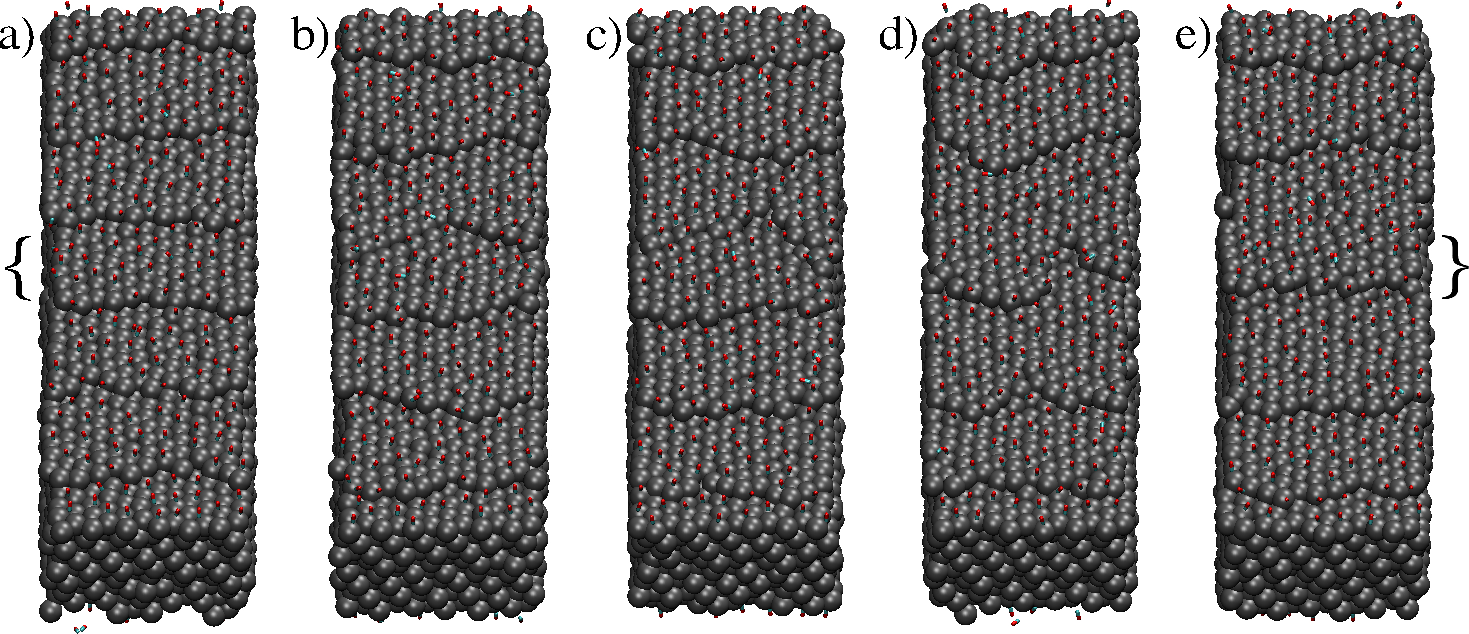
\includegraphics[width=0.9\linewidth]{../figures/appB/765MissingEdge.pdf}
\caption{The (765) MS 0.5 ML system (a) 0 ns, (b) 33.4 ns, (c) 50.2 ns, (d)
75.1 ns, (e)100 ns after exposure to CO underwent an intriguing reconstruction.
The identified step-edges in (a), approach each other while also each starting
to sink somewhat into the surface. The result in a step-edge that is between
the starting points of either parent, but still of only one atomic height.}
\label{fig:765Edge}
\end{figure}
\newpage

